\documentclass{article}
\usepackage[utf8]{inputenc}
\usepackage{geometry}
 \geometry{
 a4paper,
 total={170mm,257mm},
 left=20mm,
 top=20mm,
 }

\usepackage{
    algorithm, amssymb, booktabs, graphicx, mathtools,
    multirow, newtxtext, newtxmath, fancyvrb
}

\DeclarePairedDelimiter{\ceil}{\lceil}{\rceil}
\DeclarePairedDelimiter{\floor}{\lfloor}{\rfloor}

\title{ElGamal Experiments Report}
\author{Lucas Perin}
\date{May 2020}

\begin{document}

\maketitle

\section{Introduction}

Brett's questions:

% \begin{enumerate}
%     \item for a fixed $t$ and t-tuple $z$, are there arbitrarily large values of $p$ for which the LB from Theorem 8 is tight?
%     \item for a fixed $t$ and t-tuple $z$, are there arbitrarily large values of $p$ for which the UB from Theorem 8 is tight?
%     \item for a fixed $t$ and t-tuple $z$, are there arbitrarily large values $p$ for which $q$ is not even and the LB from Theorem 8 is tight?
%     \item for a fixed $t$ and t-tuple $z$, are there arbitrarily large values $p$ for which $q$ is not even and the UB from Theorem 8 is tight?
%     \item for a fixed $t$ and t-tuple $z$, are there arbitrarily large values $p$ for which $g$ is not even and the LB from Theorem 8 is tight?
%     \item for a fixed $t$ and t-tuple $z$, are there arbitrarily large values $p$ for which $g$ is not even and the UB from Theorem 8 is tight?
% \end{enumerate}

For a collection of primes $p$ (in millions), define a handful of primitive elements $g$ (preferably first five smallest and  10 additional spanning over the entire range). For each $g$ and with $2 \leq z \leq 15$, plot $\Delta_l = \lambda(z) - \operatorname{lower-bound}$ and $\Delta_u \operatorname{upper-bound} - \lambda(z)$.Repeat experiment with the following restrictions:

\begin{enumerate}
    \item plot only when $q$ is even;
    \item plot only when $q$ is odd;
    \item plot only when $g$ is even;
    \item plot only when $g$ is odd.
\end{enumerate}

In Theorem 8, we have that the occurrence of some arbitrary $t$-tuple in the ElGamal sequence is bounded as
$$ \floor*{\frac{g}{v}}^{t-1} \floor*{\frac{q}{v}} \leq \lambda(z) \leq \ceil*{\frac{g}{v}}^{t-1} \left(\floor*{\frac{q}{v}}+1\right).$$
We plot these bounds with the following code:
\begin{Verbatim}[frame=single]
def tuple_bound(p, v, g, t):
    """
    Bounds defined in Theorem 8 for t-tuples
    """
    q = floor(p/pow(g,t-1))
    lower = pow(floor(g/v),t-1)*floor(q/v)
    upper = pow(ceil(g/v),t-1)*(floor(q/v)+1)
    return lower, upper
\end{Verbatim}

\subsection{Expected bound explosion!}

We could probably stop plotting when (or let it happen a bit):

For the upper bound:

$$ g > \sqrt[t-1]{p}$$

$$ t > \log_g p  $$

for the lower bound:

$$ v > q $$

$$ v > g $$


\section{First Evaluating $t$-tuple bounds for $v = 2$}

In this section, we first investigated real counts and expected count with the bounds, by drawing a line over the plot. The line is truncated when the upper bound exceeds $1.3$ times the largest actual count of the entire plot. This is clear in the figures when $t$ grows. The experiments that follow do not use $\Delta_l$ or $\Delta_u$.

\subsection{Plotting all for each prime individually}

\begin{figure}[H]
    \begin{minipage}{.49\textwidth}
            \centering
            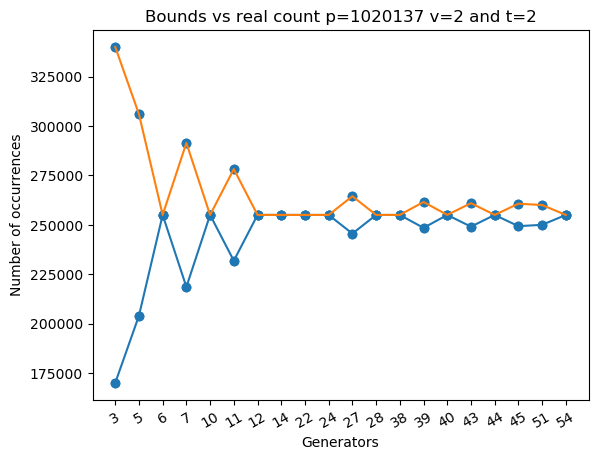
\includegraphics[width=\textwidth]{../plots/tuples_figures/1020137v2/test_p1020137_v2_t2.png}
            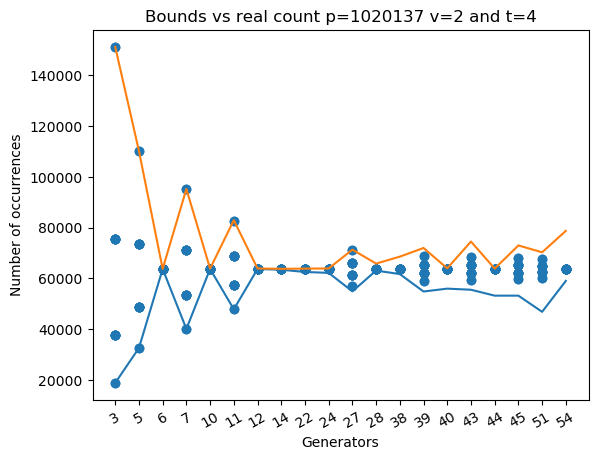
\includegraphics[width=\textwidth]{../plots/tuples_figures/1020137v2/test_p1020137_v2_t4.png}
            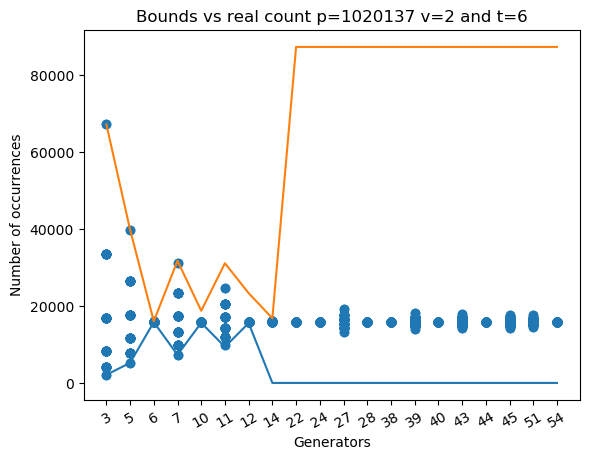
\includegraphics[width=\textwidth]{../plots/tuples_figures/1020137v2/test_p1020137_v2_t6.png}
    \end{minipage}
    \begin{minipage}{.49\textwidth}
            \centering
            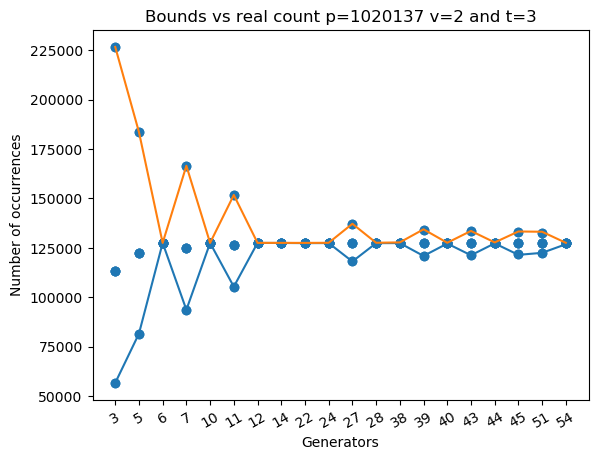
\includegraphics[width=\textwidth]{../plots/tuples_figures/1020137v2/test_p1020137_v2_t3.png}
            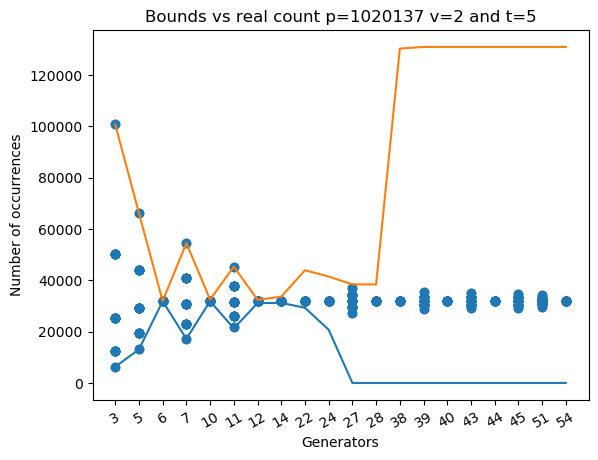
\includegraphics[width=\textwidth]{../plots/tuples_figures/1020137v2/test_p1020137_v2_t5.png}
            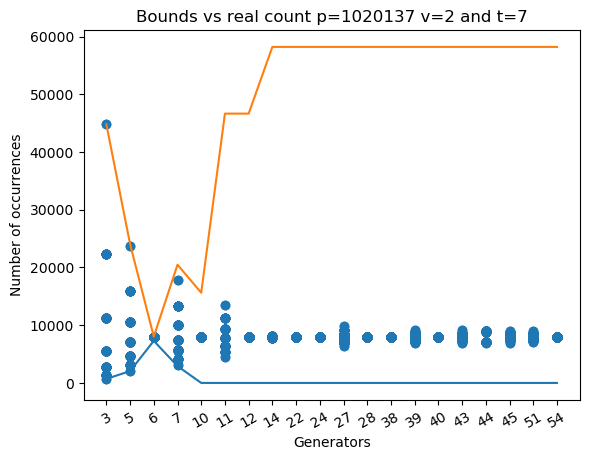
\includegraphics[width=\textwidth]{../plots/tuples_figures/1020137v2/test_p1020137_v2_t7.png}
    \end{minipage}
\end{figure}

\subsection{Plotting when $q$ is odd for each prime individually}
\begin{figure}[H]
    \begin{minipage}{.49\textwidth}
            \centering
            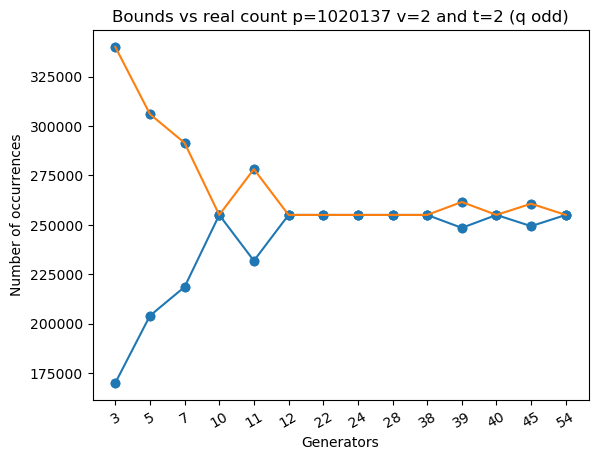
\includegraphics[width=\textwidth]{../plots/tuples_figures/1020137v2qodd/test_p1020137_v2_t2_q_odd.png}
            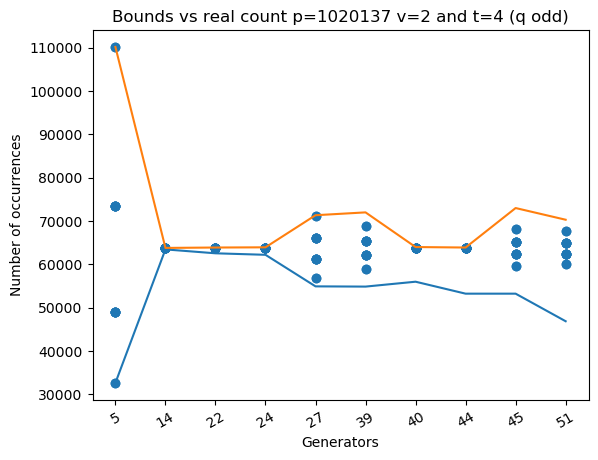
\includegraphics[width=\textwidth]{../plots/tuples_figures/1020137v2qodd/test_p1020137_v2_t4_q_odd.png}
            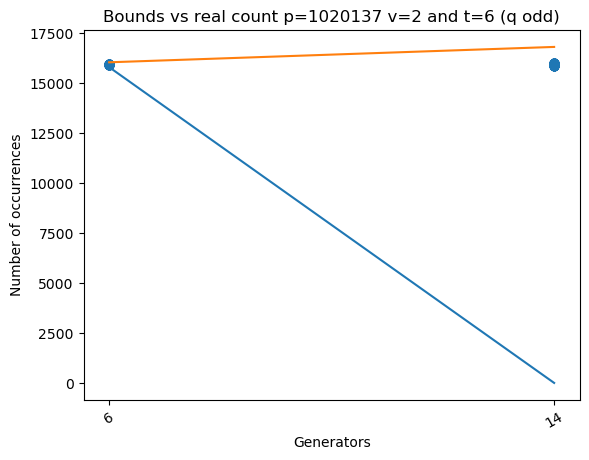
\includegraphics[width=\textwidth]{../plots/tuples_figures/1020137v2qodd/test_p1020137_v2_t6_q_odd.png}
    \end{minipage}
    \begin{minipage}{.49\textwidth}
            \centering
            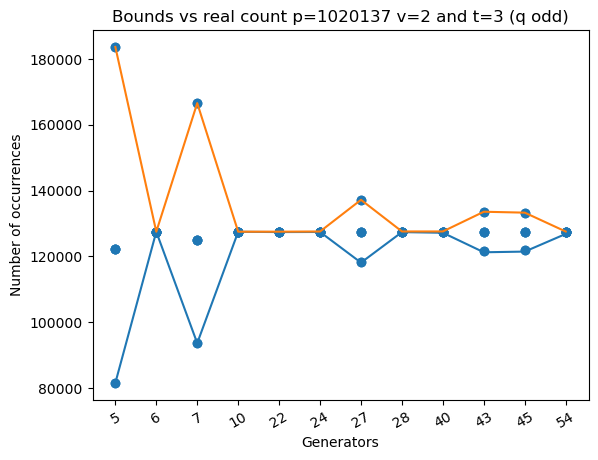
\includegraphics[width=\textwidth]{../plots/tuples_figures/1020137v2qodd/test_p1020137_v2_t3_q_odd.png}
            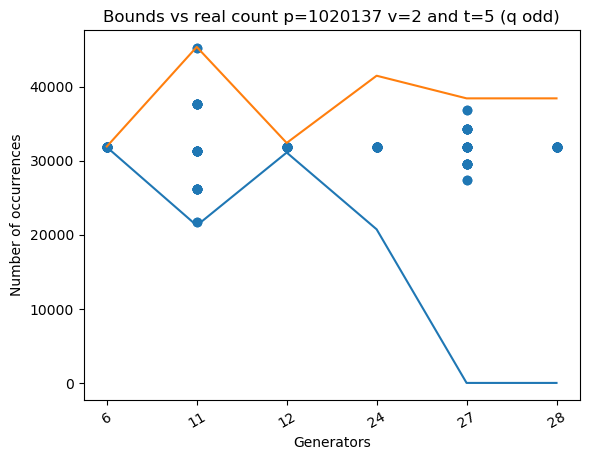
\includegraphics[width=\textwidth]{../plots/tuples_figures/1020137v2qodd/test_p1020137_v2_t5_q_odd.png}
            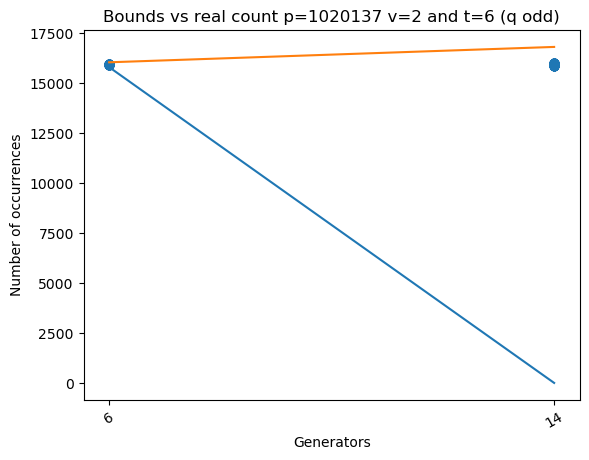
\includegraphics[width=\textwidth]{../plots/tuples_figures/1020137v2qodd/test_p1020137_v2_t6_q_odd.png}
    \end{minipage}
\end{figure}

\subsection{Plotting when $q$ is even for each prime individually}
\begin{figure}[H]
    \begin{minipage}{.49\textwidth}
            \centering
            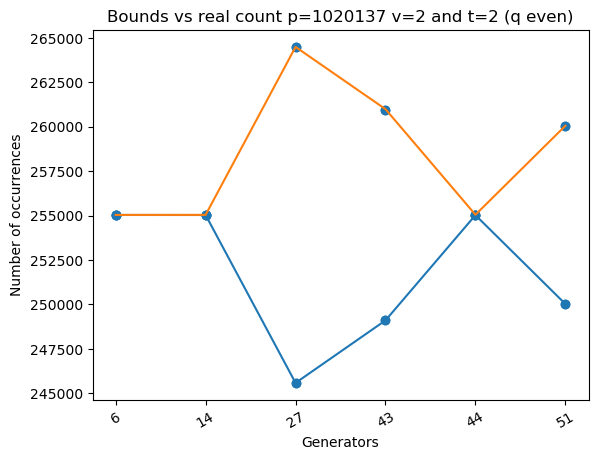
\includegraphics[width=\textwidth]{../plots/tuples_figures/1020137v2qeven/test_p1020137_v2_t2_q_even.png}
            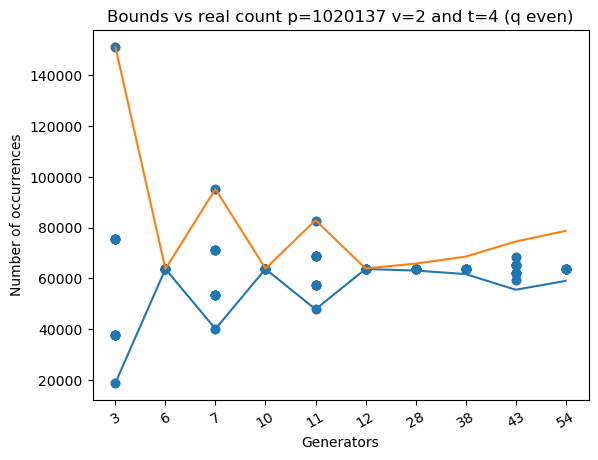
\includegraphics[width=\textwidth]{../plots/tuples_figures/1020137v2qeven/test_p1020137_v2_t4_q_even.png}
            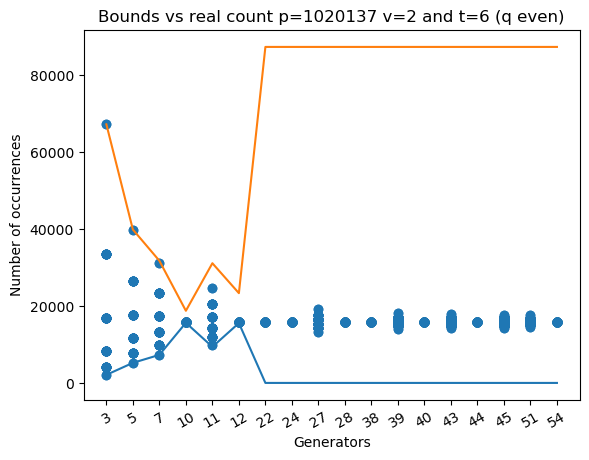
\includegraphics[width=\textwidth]{../plots/tuples_figures/1020137v2qeven/test_p1020137_v2_t6_q_even.png}
    \end{minipage}
    \begin{minipage}{.49\textwidth}
            \centering
            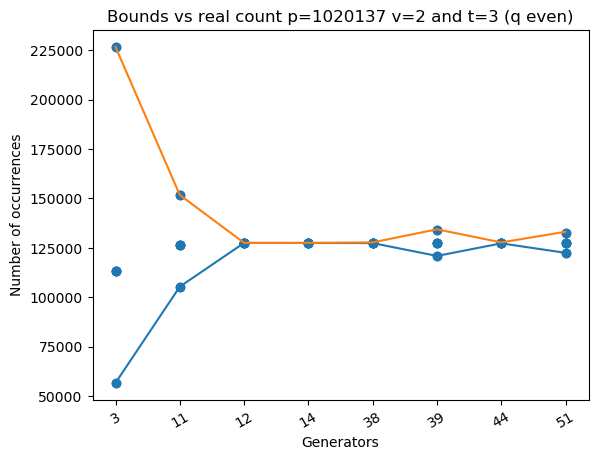
\includegraphics[width=\textwidth]{../plots/tuples_figures/1020137v2qeven/test_p1020137_v2_t3_q_even.png}
            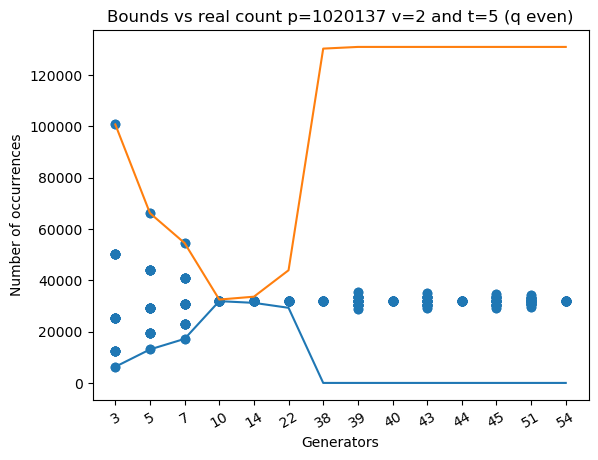
\includegraphics[width=\textwidth]{../plots/tuples_figures/1020137v2qeven/test_p1020137_v2_t5_q_even.png}
            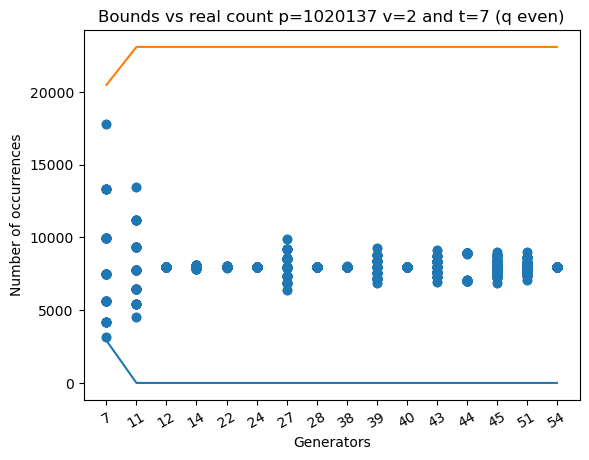
\includegraphics[width=\textwidth]{../plots/tuples_figures/1020137v2qeven/test_p1020137_v2_t7_q_even.png}
    \end{minipage}
\end{figure}

\subsection{Plotting when $g$ is odd for each prime individually}
\begin{figure}[H]
    \begin{minipage}{.49\textwidth}
            \centering
            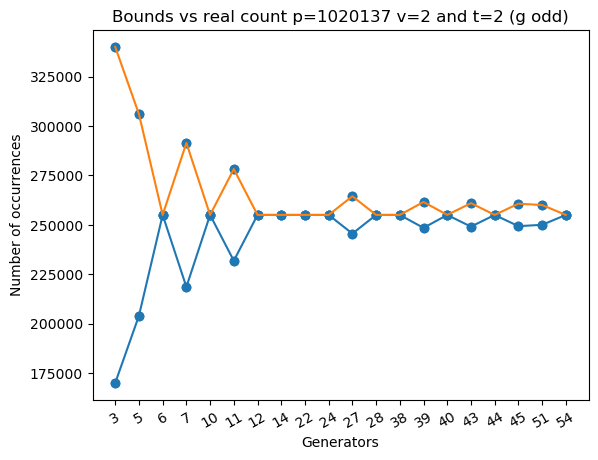
\includegraphics[width=\textwidth]{../plots/tuples_figures/1020137v2godd/test_p1020137_v2_t2_g_odd.png}
            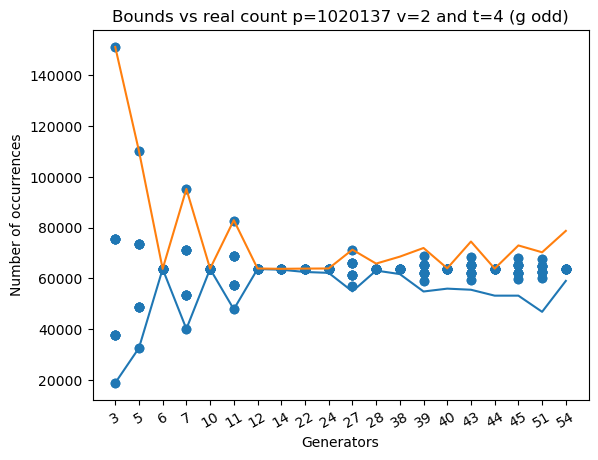
\includegraphics[width=\textwidth]{../plots/tuples_figures/1020137v2godd/test_p1020137_v2_t4_g_odd.png}
            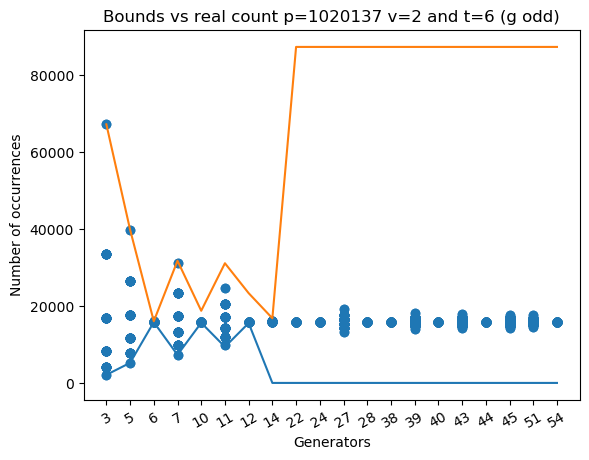
\includegraphics[width=\textwidth]{../plots/tuples_figures/1020137v2godd/test_p1020137_v2_t6_g_odd.png}
    \end{minipage}
    \begin{minipage}{.49\textwidth}
            \centering
            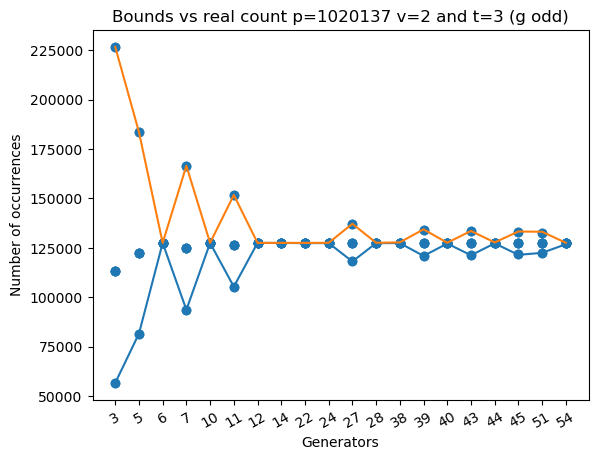
\includegraphics[width=\textwidth]{../plots/tuples_figures/1020137v2godd/test_p1020137_v2_t3_g_odd.png}
            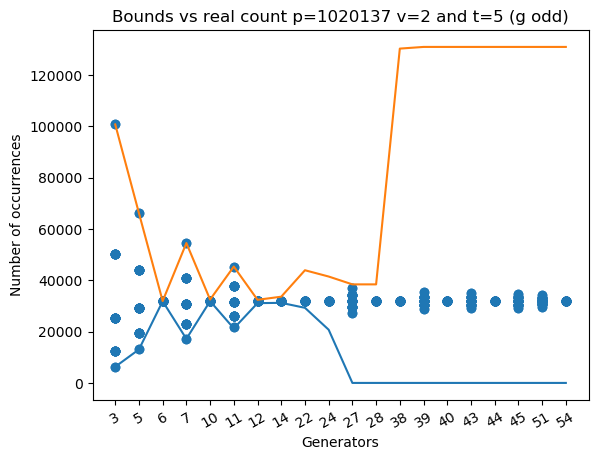
\includegraphics[width=\textwidth]{../plots/tuples_figures/1020137v2godd/test_p1020137_v2_t5_g_odd.png}
            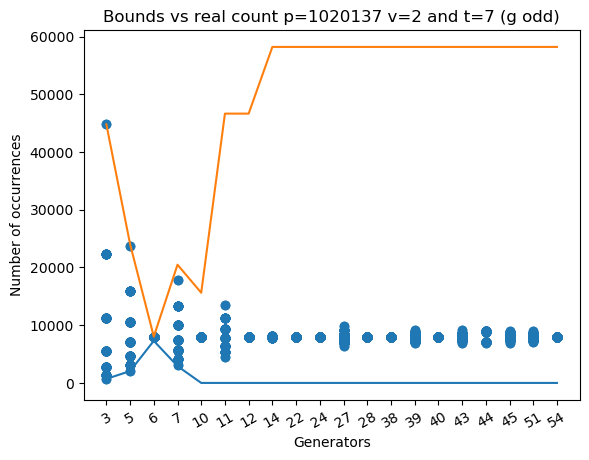
\includegraphics[width=\textwidth]{../plots/tuples_figures/1020137v2godd/test_p1020137_v2_t7_g_odd.png}
    \end{minipage}
\end{figure}

\subsection{Plotting when $g$ is even for each prime individually}
\begin{figure}[H]
    \begin{minipage}{.49\textwidth}
            \centering
            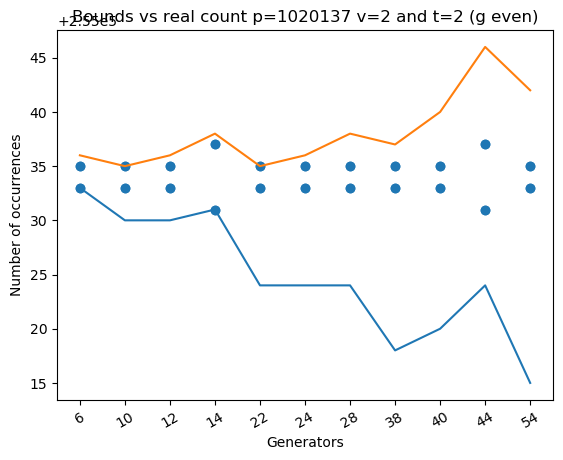
\includegraphics[width=\textwidth]{../plots/tuples_figures/1020137v2geven/test_p1020137_v2_t2_g_even.png}
            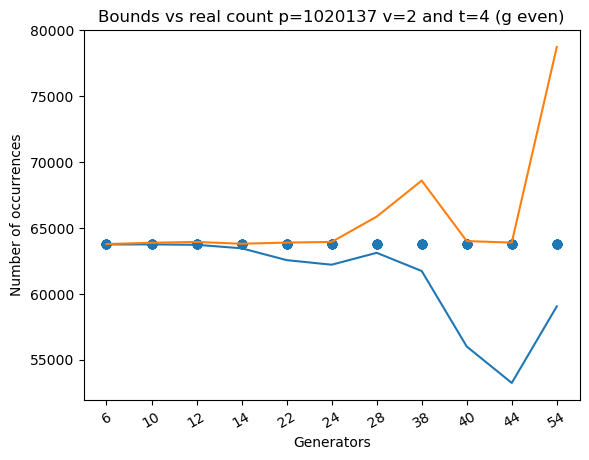
\includegraphics[width=\textwidth]{../plots/tuples_figures/1020137v2geven/test_p1020137_v2_t4_g_even.png}
            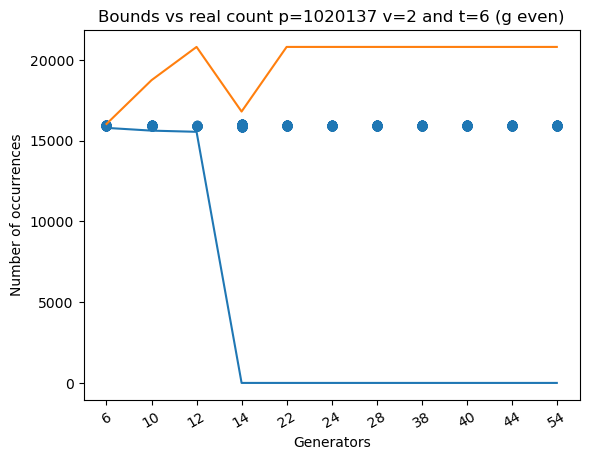
\includegraphics[width=\textwidth]{../plots/tuples_figures/1020137v2geven/test_p1020137_v2_t6_g_even.png}
    \end{minipage}
    \begin{minipage}{.49\textwidth}
            \centering
            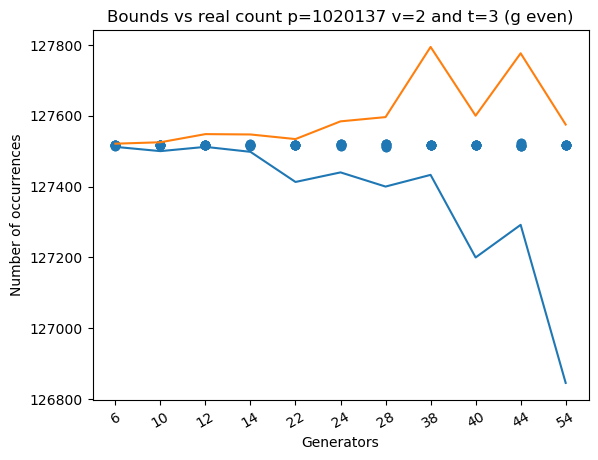
\includegraphics[width=\textwidth]{../plots/tuples_figures/1020137v2geven/test_p1020137_v2_t3_g_even.png}
            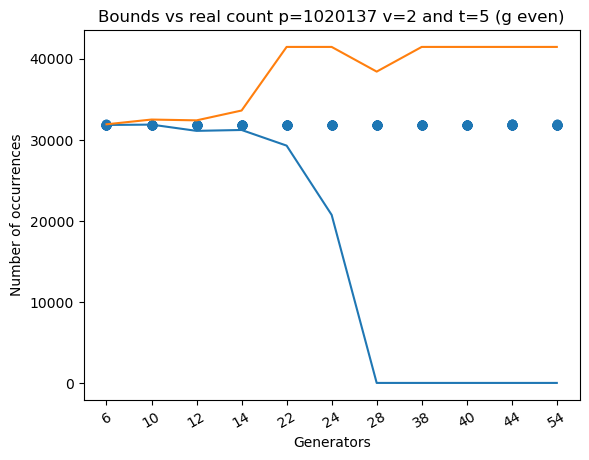
\includegraphics[width=\textwidth]{../plots/tuples_figures/1020137v2geven/test_p1020137_v2_t5_g_even.png}
            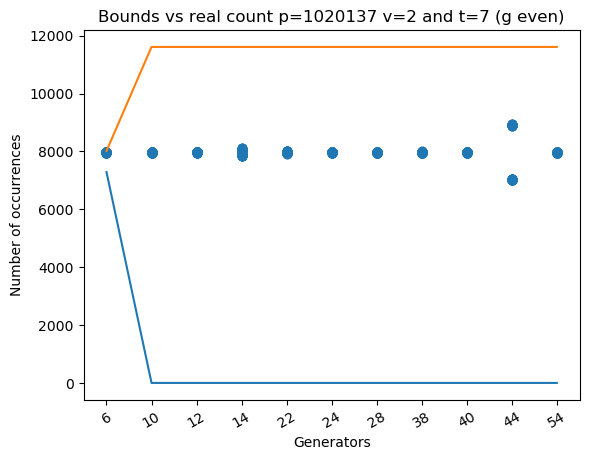
\includegraphics[width=\textwidth]{../plots/tuples_figures/1020137v2geven/test_p1020137_v2_t7_g_even.png}
    \end{minipage}
\end{figure}

\subsection{Box and 3d plots}
We may try to compose a set of experiments for the same prime all in one plot as shown below, using 3d plots. The tricky part is that the plotted data will have to be the delta mentioned in the first page --- namely, the distance of the bounds to original count. The main issue with this is that for each pair $(x,y) = (t, \lambda)$ we will have to plot two dots, one for the lower bound and one for the upper bound. Essentially, one dot may end up on top of each other or too far away, making it hard to read. I will investigate further.

\begin{figure}[H]
    \begin{minipage}{.49\textwidth}
            \centering
            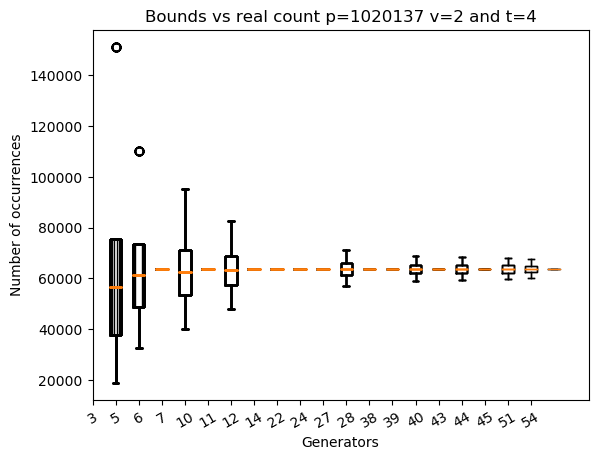
\includegraphics[width=\textwidth]{../plots/tuples_figures/other/boxplot_p1020137_v2_t4.png}
    \end{minipage}
    \begin{minipage}{.49\textwidth}
            \centering
            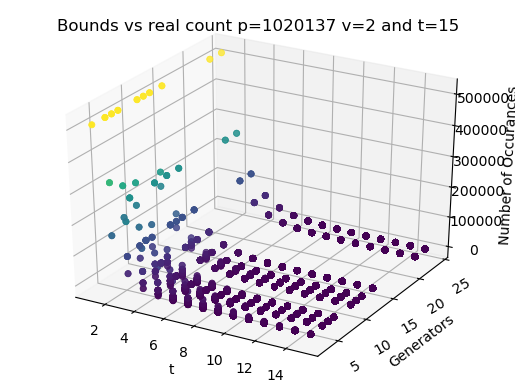
\includegraphics[width=\textwidth]{../plots/tuples_figures/other/test_p1020137_v2.png}
    \end{minipage}
\end{figure}

\section{Delta plots}

In the following, we show how the bounds have a tendency to ``explode'' for some specific set of parameters.

\begin{figure}[H]\label{fig:delta_explode}
    \begin{minipage}{.49\textwidth}
            \centering
            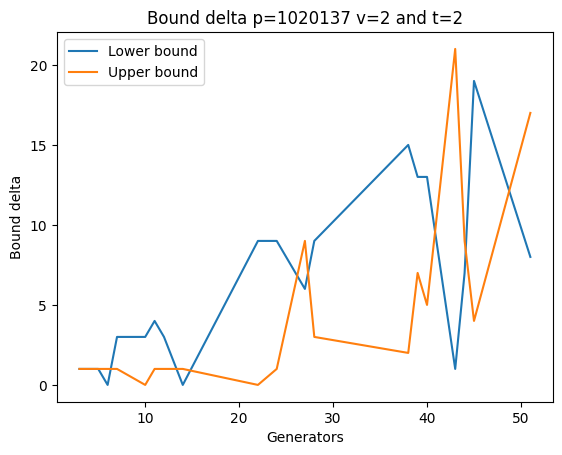
\includegraphics[width=\textwidth]{../plots/tuples_figures/delta_1020137v2_large/Bound delta p=1020137 v=2 and t=2.png}
            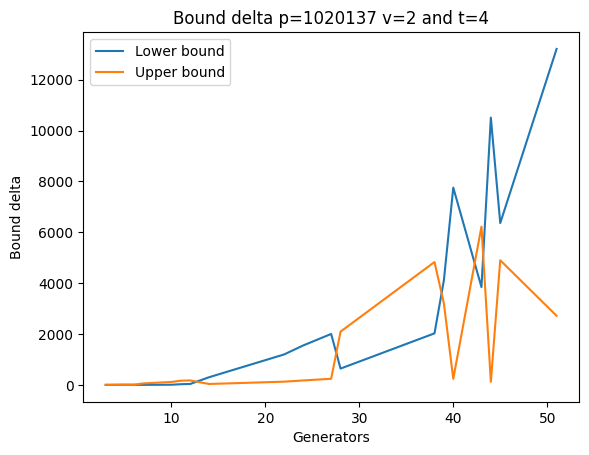
\includegraphics[width=\textwidth]{../plots/tuples_figures/delta_1020137v2_large/Bound delta p=1020137 v=2 and t=4.png}
            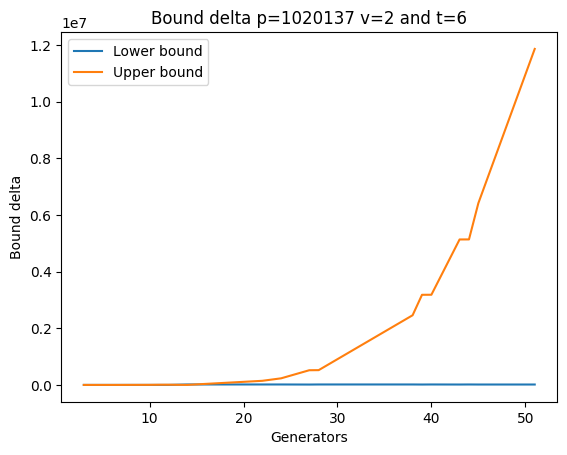
\includegraphics[width=\textwidth]{../plots/tuples_figures/delta_1020137v2_large/Bound delta p=1020137 v=2 and t=6.png}
    \end{minipage}
    \begin{minipage}{.49\textwidth}
            \centering
            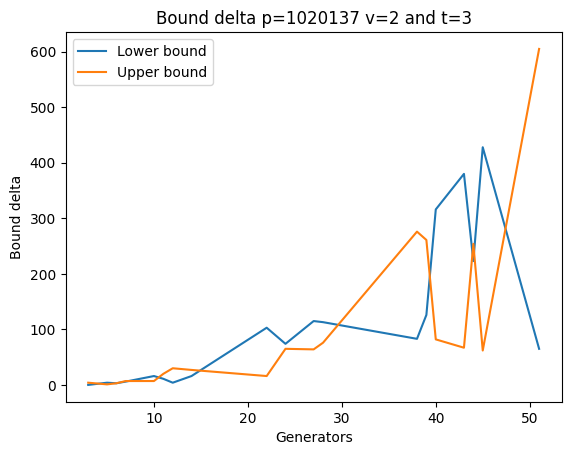
\includegraphics[width=\textwidth]{../plots/tuples_figures/delta_1020137v2_large/Bound delta p=1020137 v=2 and t=3.png}
            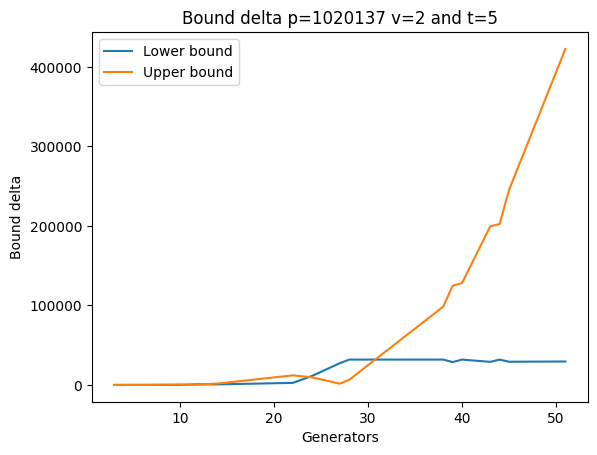
\includegraphics[width=\textwidth]{../plots/tuples_figures/delta_1020137v2_large/Bound delta p=1020137 v=2 and t=5.png}
            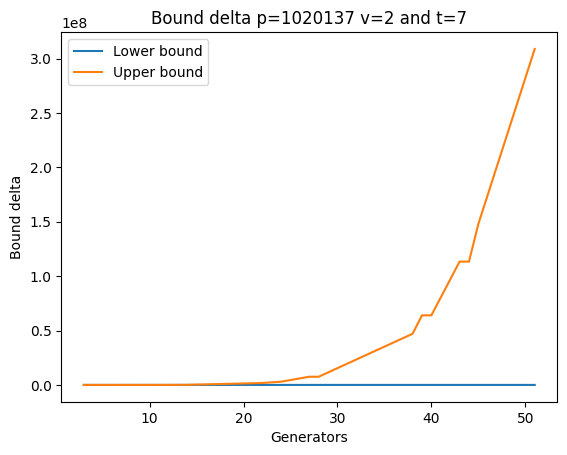
\includegraphics[width=\textwidth]{../plots/tuples_figures/delta_1020137v2_large/Bound delta p=1020137 v=2 and t=7.png}
    \end{minipage}
\end{figure}

\subsection{Tight delta plots}

Now, we present plots for parameter sets where the bounds are tight, that is, close to the actual count. We do this by considering only parameters such that, for small $v$, $g < \lfloor \sqrt[t-1]{p} \rfloor$ and $t < \lfloor log_g p \rfloor $. For example, let $(t, p, v) = (7, 1020137, 2)$, then we are we have that the bound explodes when $g \geq 10$. The same happens if we set $t = 5$ for $g >= 31$.

\begin{figure}[H]
    \begin{minipage}{.49\textwidth}
            \centering
            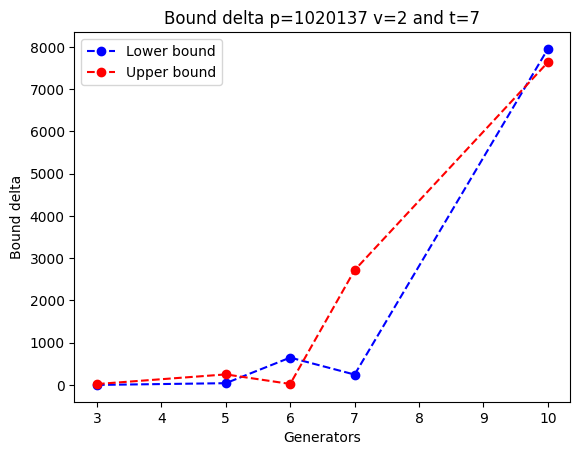
\includegraphics[width=\textwidth]{../plots/tuples_figures/explosion_example.png}
    \end{minipage}
    \begin{minipage}{.49\textwidth}
            \centering
            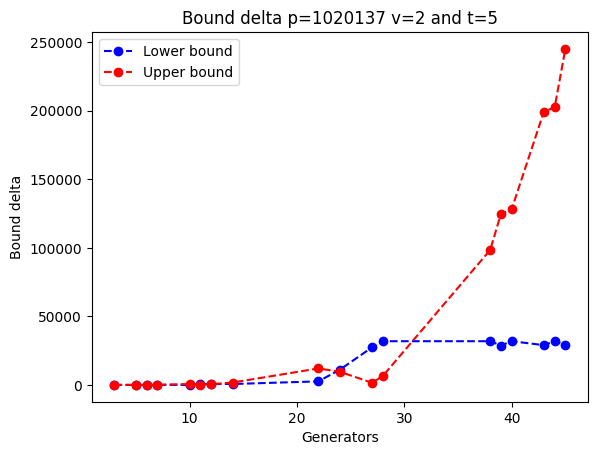
\includegraphics[width=\textwidth]{../plots/tuples_figures/explosion_example_2.png}
    \end{minipage}
\end{figure}


As it shows in the examples, these parameter constraints do not correlate to the explosion of the lower bound necessarily. Clearly, since the lower bound cannot be less than zero, eventually it will be stable. However, we do expect it \emph{NOT} to be tight when $v > q$ or $v > g$. While the first requires $v$ to be large when $p$ grows, the second is may occur eventually (even as $p$ grows) for small value $v$. Observe the following display of this behaviour.
\begin{figure}[H]
    \begin{minipage}{.49\textwidth}
            \centering
            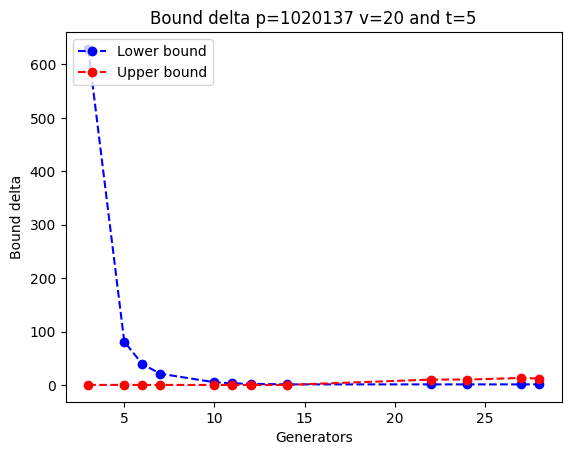
\includegraphics[width=\textwidth]{../plots/tuples_figures/explosion_example_3.png}
    \end{minipage}
    \begin{minipage}{.49\textwidth}
            \centering
            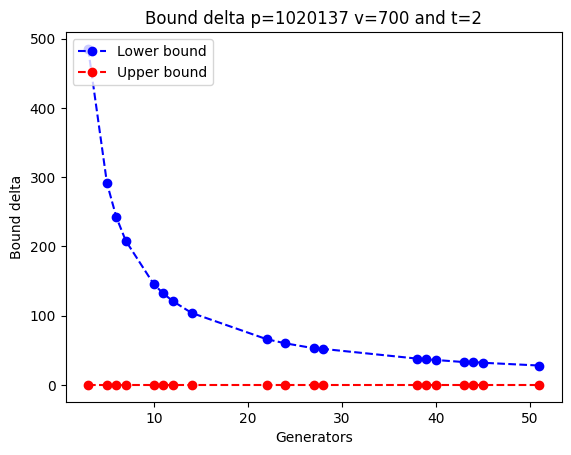
\includegraphics[width=\textwidth]{../plots/tuples_figures/explosion_example_4.png}
    \end{minipage}
\end{figure}

We also remark that the numbering on the $y$ axis makes it difficult to actually understand how tight the bound is. One would always consider the $\Delta$ close to zero to be tight, and zero to be exact. But when $\lambda(z)$ varies in range of hundreds of thousands, looking at $\Delta$ in range of thousands is not so bad. Let us look at the same examples but using a ratio value.

\begin{figure}[H]
    \begin{minipage}{.49\textwidth}
            \centering
             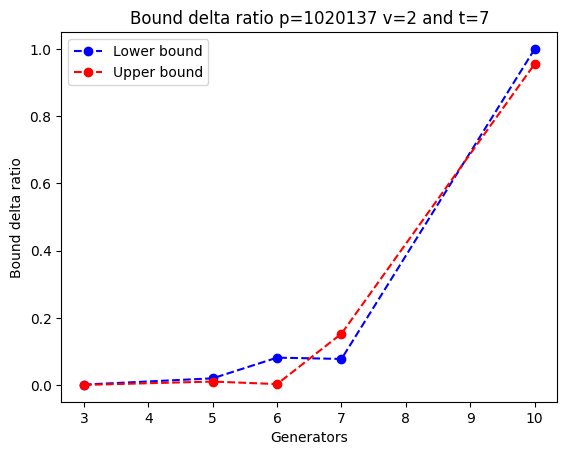
\includegraphics[width=\textwidth]{../plots/tuples_figures/explosion_example_1.2.png}
             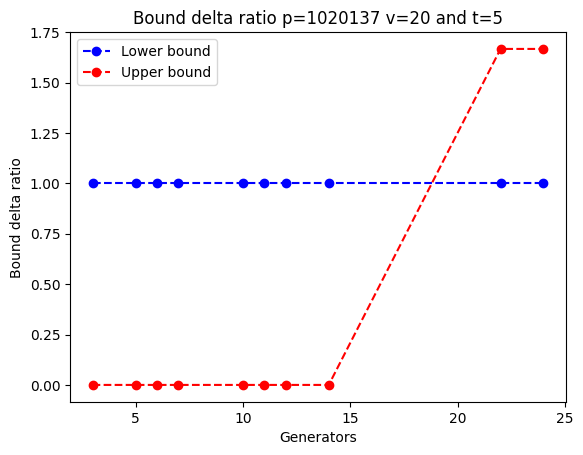
\includegraphics[width=\textwidth]{../plots/tuples_figures/explosion_example_3.2.png}
    \end{minipage}
    \begin{minipage}{.49\textwidth}
            \centering
            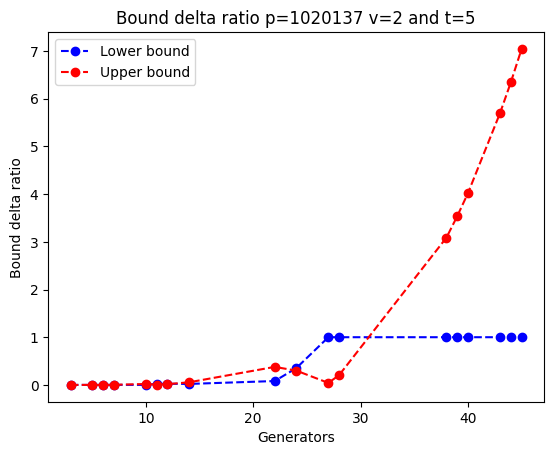
\includegraphics[width=\textwidth]{../plots/tuples_figures/explosion_example_2.2.png}
            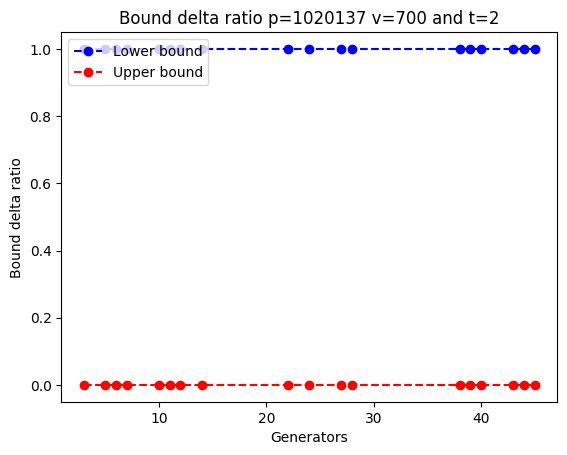
\includegraphics[width=\textwidth]{../plots/tuples_figures/explosion_example_4.2.png}
    \end{minipage}
\end{figure}

Brett and Daniel. These last two plots are weird. What happens here is that the lower bound is zero but the actual count is not. Let $\Delta_l$ denote the difference of actual count and the lower bound, namely $\min(\lambda(z)) - lb$, then I compute the ratio as follows:
$$ \Delta_l^r = \frac{\min(\lambda(z)) - lb/}{\min(\lambda(z))} = 1 - \frac{lb}{\min(\lambda(z)}$$ 
and for the upper bound $\Delta_u$
$$ \Delta_u^r = \frac{ub - \max(\lambda(z))}{\max(\lambda(z))} = \frac{ub}{\max(\lambda(z))} - 1 $$

This means that this ratio is bad when it comes to show the lower bound. Any tips?
\end{document}
